% % % % % % % % % % % % % % % % % % % % % % % % % % % % % % % % % % % % % % % % 
% LaTeX4EI Template for Cheat Sheets                                Version 1.0
%					
% Authors: Emanuel Regnath, Martin Zellner
% Contact: info@latex4ei.de
% Encode: UTF-8, tabwidth = 4, newline = LF	
% % % % % % % % % % % % % % % % % % % % % % % % % % % % % % % % % % % % % % % % 


% ======================================================================
% Document Settings
% ======================================================================

% possible options: color/nocolor, english/german, threecolumn
% defaults: color, english
\documentclass[german]{latex4ei/latex4ei_sheet}
\usepackage{stix}
\usepackage[ngerman]{babel} 
% set document information
\title{Leistungselektronik \\ Cheat Sheet}
\author{Raoul Duke}
\myemail{0x4723@gmail.com}
\mywebsite{www.github.com/doppelplus/CheatSheets}

% ======================================================================
% Define MathOperator
% ======================================================================

\DeclareMathOperator{\arcsec}{arcsec}
\DeclareMathOperator{\arccot}{arccot}
\DeclareMathOperator{\arccsc}{arccsc}
\DeclareMathOperator{\arcsinh}{asinh}
\DeclareMathOperator{\arccoth}{acoth}
\DeclareMathOperator{\arctanh}{atanh}
\DeclareMathOperator{\arccosh}{acosh}

% ======================================================================
% Begin
% ======================================================================
\begin{document}


% Title
% ----------------------------------------------------------------------
\maketitle   % requires ./img/Logo.pdf

% Tipps und Tricks
% ----------------------------------------------------------------------
\section{Allgemeines}
	\begin{sectionbox}
		\begin{symbolbox}{Allgemeines}
			\item Tastverhältnis: $D = \frac{\tau_i}{T}$
			\item Funktion einer Sinusspannung: $u(t) = \hat{U_s} \cdot \sin(\omega t)$
		\end{symbolbox}
		\begin{bluebox}{Physikalische Größen}
			\item $U_0$: Gleichspannung
			\item $\hat{u}$: Scheitelwert
			\item $u(t)$: zeitabhängige Spannung
			\item $T$: Periodendauer
			\item $t_i$: Impulszeit
			\item $\overline{U}$: Arithmetischer Mittelwert
		\end{bluebox}
	\end{sectionbox}
\section{Mathematische Verfahren}
	\subsection{Mittel- \& Effektivwert}
	\begin{sectionbox}
		\begin{symbolbox}
			\item Arith. Mittelwert einer Mischspannung: $\overline{u}_{di} = U_{di} = \frac{1}{T}\int\limits_0^T u_d(t)\,dt$
			\item Effektivwert: $U_{RMS} = \sqrt{\frac{1}{T}\cdot \int\limits_0^T u^2_d(t)\,dt}= \sqrt{\frac{1}{2\pi}\cdot \int\limits_0^{2\pi} u^2_d(\omega t)\,d\omega t}$
		\end{symbolbox}
		\begin{cookbox}{Effektivwert einer diskreten Spannung}
			\item Spannung in Spannungen mit gleichem $\hat{U}$ aufteilen.
			\item Effektivwerte der Einzelspannungen berechnen:\\ $U_{xRMS} = \sqrt{D} \hat{U}$.
			\item Quadratische Summe aller $U_{xRMS}$ berechnen: $\\ U_{RMS} = \sqrt{U_{xRMs}^2+U_{x+1RMs}^2\dots}$
		\end{cookbox}
	\subsection{Welligkeit, Klirr und Formfaktor}
		\begin{symbolbox}{Welligkeit (Ripple)}
			\item $w_U = \frac{U_{RMS}}{U_d} = \sqrt{\frac{U_{RMS\,ges}^2}{U_d^2}-1}$
			\item $w_I = \frac{I_{RMS}}{I_d} = \sqrt{\frac{I_{RMS\,ges}^2}{I_d^2}-1}$
			\item Welligkeit reiner Gleichgrößen: $w = 0$.
			\item Welligkeit reiner Wechselgrößen: $w =$ sehr groß.
		\end{symbolbox}
		\begin{bluebox}{Klirrfaktor (THD)}
			\item $K_U =   \frac{U_{RMS\, OS}}{U_{RMS}}$
			\item $K_I =   \frac{I_{RMS\, OS}}{I_{RMS}}$
		\end{bluebox}

		\begin{symbolbox}{Formfaktor}
			\item $F = \frac{U_{d\,RMS}}{U_{di}}$
		\end{symbolbox}
	\end{sectionbox}
	\vspace{3cm}
\section{Leistungsberechnung}
	\begin{sectionbox}
		\subsection{Leistungsarten}
			\begin{bluebox}
				\item 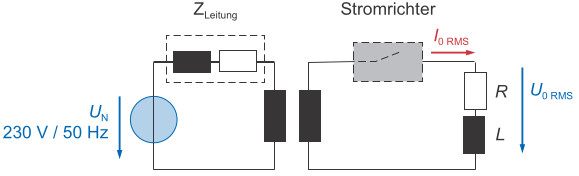
\includegraphics[width=180px]{img/Leistungsarten.png}
				\item $S = U_{0\,RMS} \cdot I_{O\,RMS}$
				\item Für rein sinusförmige Verläufe gilt:
				\item $\lambda = \frac{P}{S} = \cos \phi$
				\item $S = \sqrt{P^2+Q^2}$
				\item $Q = \sin(\phi)$
			\end{bluebox}
		\subsection{Betriebsquadranten}
			\begin{symbolbox}
				\item 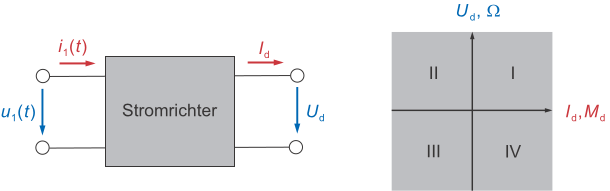
\includegraphics[width=180px]{Betriebsquadranten.png}
			\end{symbolbox}
	\end{sectionbox}
\section{Wärmemanagement}
	\begin{sectionbox}
		\subsection{Verlustleistung}
			\begin{bluebox}
				\item Thermische Energie: Q
				\item Momentanleistung am PN Übergang: $p_v = u \cdot i$
				\item $Q = \int\limits_0^t p(t)\,dt$
				\item 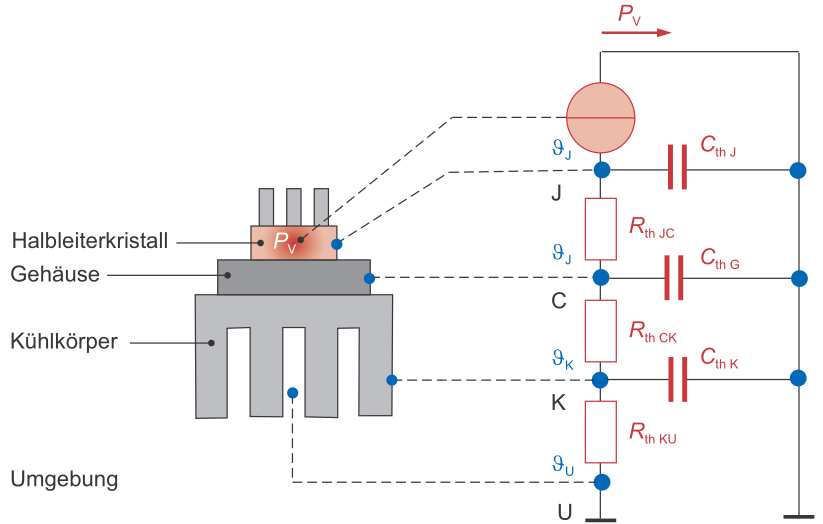
\includegraphics[width=180px]{TempErsatzschaltbild.png}
			\end{bluebox}
			\begin{tabular}{|l|c|c|}
				\textbf{Bauelement}	& \textbf{Kennbuchstabe} & \textbf{Temperatur}\\
				\hline
				Siliziumkristall - Junction & J & $\vartheta_J$\\
				Gehäuse - case & C & $\vartheta_C$\\
				Kühlkörper - heatsink & K & $\vartheta_K$\\
				Kühlmedien - ambient & U / A & $\vartheta_A$
				
			\end{tabular}
	\end{sectionbox}
	\vspace{3cm}
\section{Mittelpunktschaltungen}
	\begin{sectionbox}
		\subsection{Nomenklatur}
			\begin{bluebox}
				\item $i_d\,u_d$: Zeitverläufe von Strom und Spannung
				\item $I_d\,U_d$: In den Zeitverläufen von $i_d$ und $u_d$ enthaltene Mittelwerte
				\item $u_T$: Zeitlicher Verlauf der Spannung an einem Thyristor
				\item $u_S$: Zeitlicher Verlauf der Netzspannung
				\item $U_S$: Effektivwert der Netzspannung
				\item $U_N$: Effektivwert der verketteten Spannung
				\item $d$: Ausgangsgröße
				\item $T$: Transistor
				\item $S$: Strang
				\item $N$: verkettet Größe
			\end{bluebox}
		\subsection{Welligkeit}
			\begin{bluebox}
				\item $w_U = \sqrt{\frac{U_{RMS}^2}{U_d^2}-1}$
			\end{bluebox}
		\subsection{Einphasige Mittelpunktschaltung M1}
			\subsubsection{Aufbau und Funktion}
				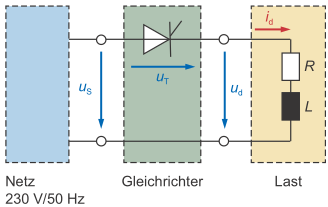
\includegraphics[width=110px]{Mittelpunktschaltung.png}
			\subsubsection{Steuergesetz}
					Rein ohmsche Last: $U_{di\alpha} = \frac{\hat{U}_S}{2\pi}\cdot (1+\cos  \alpha)$

					$\frac{U_{di\alpha}}{U_{di0}} = \frac{1+\cos \alpha}{2}$

		\subsection{Zweiphasige Mittelpunktschaltung M2C}
			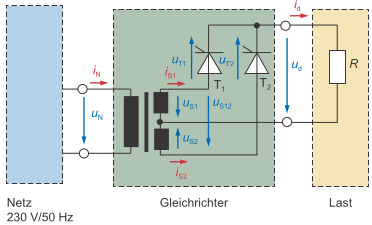
\includegraphics[width=110px]{ZweiphasigeMittelpunktschaltung.png}

			$u_{s12} = u_{s1}-u_{s2} = u_N \cdot \frac{N_2}{N_1}$
			\subsubsection{Stromglättung}
				Bei induktiver Last gilt: $u_d = u_R + u_L = i_d\cdot R+L\cdot \frac{di_d}{dt}$
			\subsubsection{Steuergesetz}
				Bei nicht lückendem Betrieb ergibt sich für $U_{di\alpha}$:

				$U_{di\alpha} = \frac{1}{2\pi}\int\limits_\alpha^{2\pi+\alpha}u_d(\omega t)d(\omega  t) = \frac{2\cdot \sqrt{2}}{\pi}\cdot \hat{U}_S \cdot \cos \alpha$
		\subsection{Dreiphasige Mittelpunktschaltung M3C}
			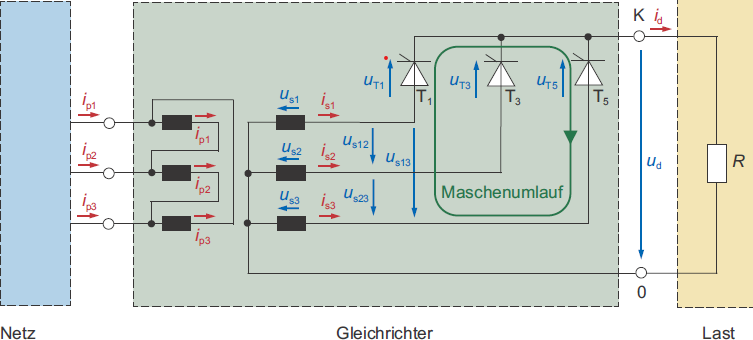
\includegraphics[width=120px]{M3C.png}

			$U_{RMS} = \hat{U}_S \sqrt{\left[ \frac{1}{2}+\frac{3}{4\pi}\cdot \frac{\sqrt{3}}{2}\right]} = 0,8405\cdot \hat{U}_S$
			\subsubsection{Steuergesetz}
			$U_{di\alpha} = \frac{3\cdot \sqrt{3}\cdot \hat{U_s}}{2\pi}\cdot \cos \alpha = \frac{3\cdot \sqrt{3}\cdot \sqrt{2}\cdot U_{s}}{2\pi} \cdot \cos \alpha$

	\end{sectionbox}
\section{Gleichstromsteller im Einquadrantenbetrieb}
	\begin{sectionbox}
		Prinzipieller Aufbau Gleichstromsteller

		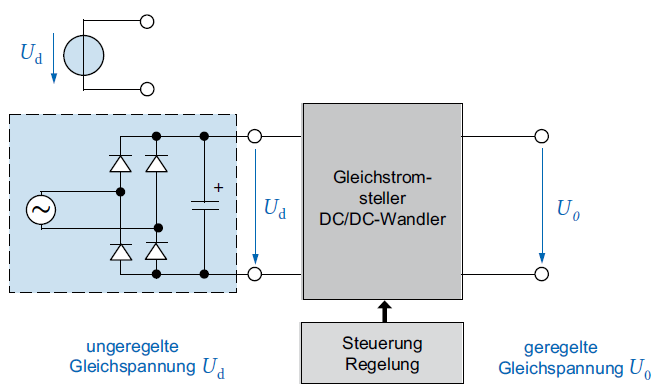
\includegraphics[width=120px]{DCSteller.png}
		\subsection{Tiefsetzsteller}
			\begin{bluebox}
				\item 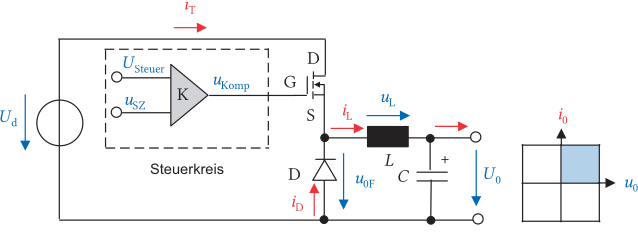
\includegraphics[width=160px]{Tiefsetzsteller.png}
				\item $u_{SZ}(t) = \frac{\hat{U}_{SZ}}{T_S}\cdot t = U_{Steuer}$
				\item $\frac{\hat{U}_{SZ}}{T_S}\cdot t_{ein} = U_{Steuer}$
				\item $t_{ein} = \frac{U_{Steuer}}{\hat{U}_{SZ}}\cdot T_S$
				\item 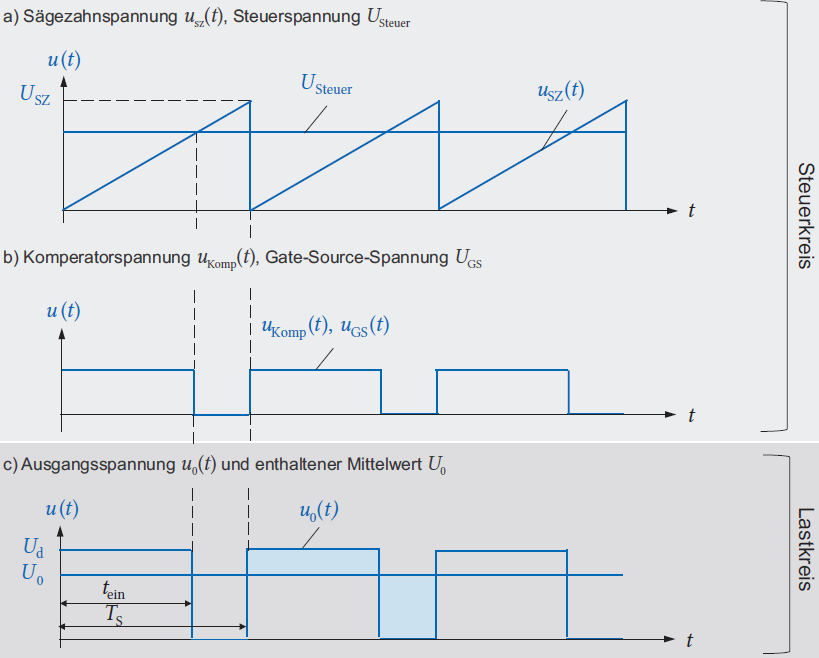
\includegraphics[width=160px]{ZeitverlaufTiefsetzsteller.png}
				\item Tastgrad: $D = \frac{t_{Ein}}{T_S}$
				\item Schaltbedingung:
				\item $u_{Komp} > 0 \Rightarrow $ MOSFET eingeschaltet $u_0(t) = U_d$
				\item $u_{Komp} < 0 \Rightarrow $ MOSFET ausgeschaltet $ u_0(t) = 0$
				\item Mittelwert der Ausgangsspannung: $U_0 = \frac{t_{ein}}{T_S}\cdot U_d = D \cdot U_d$
				\item $T_S = \frac{1}{f_S}$
				\item $t_{Ein} = \frac{U_{Steuer}}{\hat{U}_{SZ}}\cdot T_S$
				\item Resonanzfrequenz: $f_C = \frac{1}{2\pi \sqrt{L\cdot C}}$
				\item L und C sind so zu wählen: $f_C/f_S = 0,01\Rightarrow \frac{1}{2\pi\sqrt{L\cdot C}} = 0,01\cdot f_S$
				\item Stromwelligkeit: $\Delta_{iL} = \frac{u_L}{L}\cdot t_{ein} = \frac{U_d-U_0}{L}\cdot t_{ein}$
			\end{bluebox}
			\subsubsection{Lückender Betrieb}
				\begin{bluebox}
					\item $I_{Lg} = \frac{1}{2}\cdot i_{L\,peak} = \frac{t_{ein}}{2L}\cdot (U_d-U_0) = \frac{D\cdot T_S}{2L}\cdot (U_d-U_0) = I_{0g}$
					\item $\frac{U_0}{U_D} = \frac{D^2}{D^2+\frac{1}{4}\cdot \frac{I_0}{I_{L\,gmax}}}$
					\qquad $D = \frac{U_0}{U_d}\cdot \sqrt{\frac{\frac{I_0}{I_{L\,gmax}}}{1-\frac{U_0}{U_d}}}$
				\end{bluebox}	
	\end{sectionbox}
	\begin{sectionbox}
		\subsection{Hochsetzsteller}
			\begin{bluebox}
				\item 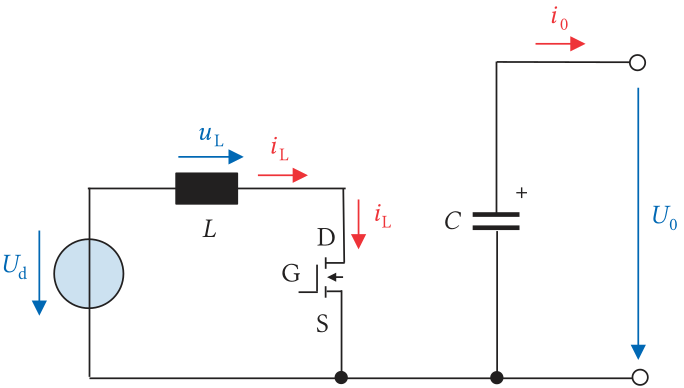
\includegraphics[width=160px]{Hochsetzsteller.png}
				\item Der Mittelwert der Ausgangsspannung $U_0$ ist höher als der Mittelwert der Eingangsspannung $U_d$.
				\item $U_d = U_L = L \cdot \frac{di_L}{dt}$
				\item $i_L = \int U_d\,dt = \frac{U_d}{L}\cdot t = \frac{(U_d-U_0)}{L}\cdot t$
				\item 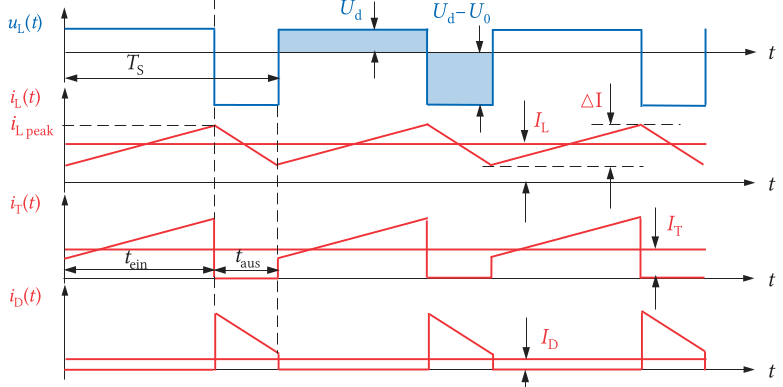
\includegraphics[width=180px]{ZeitverlaufHochsetzsteller.png}
				\item $\frac{U_0}{U_d} = \frac{T_S}{T_S-t_{ein}} = \frac{1}{1-D}$
			\end{bluebox}
			\subsubsection{Lückender Betrieb}
				\begin{bluebox}
					\item $I_{Lg} = \frac{1}{2}\cdot i_{L\,peak} = \frac{t_{ein}}{2L}\cdot U_d = \frac{D}{2L}\cdot T_S\cdot U_d = \frac{T_S}{2L}\cdot D \cdot U_0 \cdot (1-D)^2$
					\item 
				\end{bluebox}
	\end{sectionbox}
\section{Gleichstromsteller im Zweiquadrantenbetrieb}
	\begin{sectionbox}
		\subsection{Zweiquadrantensteller mit Stromumkehr}
			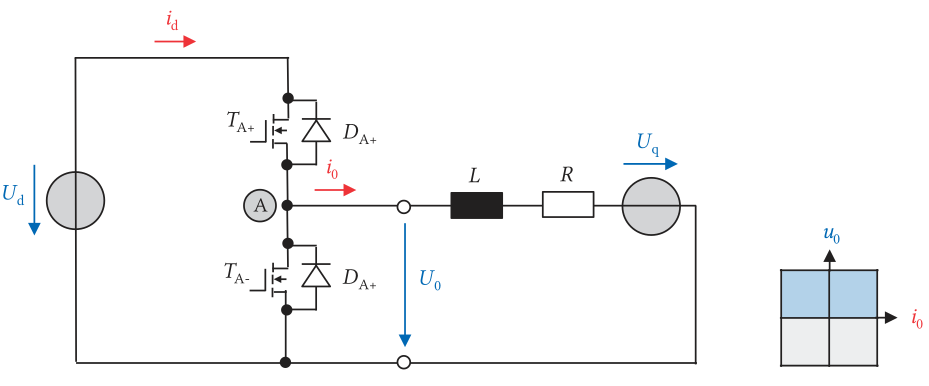
\includegraphics[width=180px]{ZweiquadrantenstellerStromumkehr.png}
		\subsection{Zweiquadrantensteller mit Spannungsumkehr}
			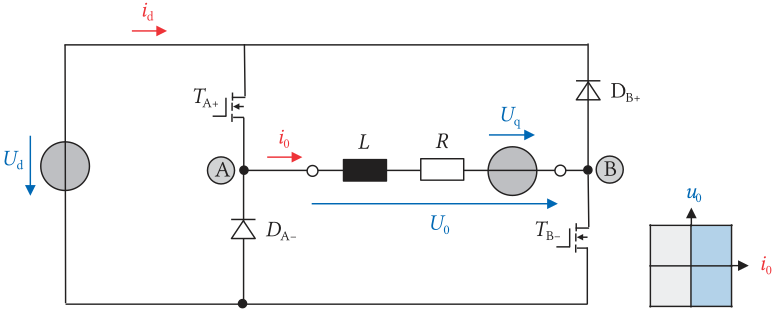
\includegraphics[width=180px]{ZweiquadrantenstellerSpannungsumkehr.png}

	\end{sectionbox}
% ======================================================================
% End
% ======================================================================
\end{document}